\documentclass[11pt]{article}

% Color package
\usepackage{xcolor}

% Color scheme definitions
\definecolor{minimal-main}{HTML}{131313}
\definecolor{minimal-light}{HTML}{F2F2F2}
\definecolor{minimal-contrast}{HTML}{F3F2F5}
\definecolor{minimal-black}{HTML}{131313}
\definecolor{minimal-white}{HTML}{F3F2F5}
\definecolor{minimal-red}{HTML}{C43C2D}
\definecolor{minimal-blue}{HTML}{343454}
\definecolor{minimal-yellow}{HTML}{F1C40F}

% Colorbox environments
\usepackage[most]{tcolorbox}

% Page layout (A4)
\usepackage[paperheight=842pt, paperwidth=595pt, margin=0pt]{geometry}

% Remove paragraph indentation
\setlength{\parindent}{0pt}

% Interline spacing options
\newcommand{\largespace}{\\[2pt]}
\newcommand{\mediumspace}{\\[-3pt]}
\newcommand{\smallspace}{\\[-5pt]}

% In-box spacing around content
\newcommand{\inboxspacing}{.015\paperheight}

% Horizontal spacing of the boxes (must sum up to 1)
\newcommand{\sideboxwidth}{.35}
\newcommand{\mainboxwidth}{.65}

% Vertical spacing of the boxes (must sum up to 1)
\newcommand{\headboxheight}{.080}
\newcommand{\sideboxheight}{.910}
\newcommand{\aboutboxheight}{.120}
\newcommand{\mainboxheight}{.800}
\newcommand{\footboxheight}{.010}

% Typesetting packages
\usepackage[letterspace=20]{microtype}
\usepackage[T1]{fontenc}

% Raleway font family
\usepackage[semibold]{raleway}
\renewcommand{\familydefault}{\sfdefault}

% Custom font commands
\newcommand{\header}[2]{\uppercase{\textbf{\fontsize{30}{100}{\lsstyle{#1 \hspace{3pt} #2}}}}}
\newcommand{\titlefont}[1]{\uppercase{\textbf{\Large{#1}}}}

% Multirow tables
\usepackage{multirow}

% Settings for entire table columns
\usepackage{array}

% Tikzpicture graphics
\usepackage{tikz}

% Clickable URLs
\usepackage{hyperref}
\urlstyle{same}

% Expand span of tables
\usepackage{tabularx}

\begin{document}

\begin{tcbposter}[
    poster = {columns=1, rows=1, spacing=0pt},
    boxes = {sharp corners, halign=center, valign=center, boxrule=0pt}
]


% -- Headbox

\posterbox[
    colback=minimal-main,
    halign=center]
    {name=headbox,
    span=1,
    rowspan=\headboxheight}
{

    \color{white}

    \header{Mario}{Gonzalez}

    \vspace{-7px}
    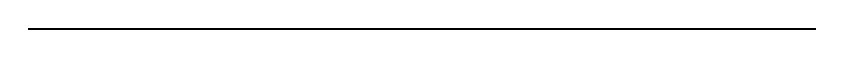
\begin{tikzpicture}
        \draw[fill=white] (-5.0, -0.01) rectangle (5.0, 0.01);
    \end{tikzpicture}
    \vspace{5px}

    \titlefont{Sofware \& Hardware Engineering}
}


% -- Sidebox
\posterbox[
    colback=minimal-light,
    valign=top,
    top=\inboxspacing,
    halign=left,
    right=\inboxspacing]
    {name=sidebox,
    below=headbox,
    column=1,
    span=\sideboxwidth,
    rowspan=\sideboxheight}
{
    \begin{tabular}{rl}
        \multicolumn{2}{@{}c@{}}{
\includegraphics[scale=0.25]{images/pic.png}} \\
        \mediumspace

        & \titlefont{Contact} \\
        \hline \mediumspace

        \multirow{4}{*}{\scalebox{0.075}{
\begin{tikzpicture}

    % Clip mask
    \clip (0, 0) circle (7);

    % Background
    \fill[minimal-red] (-7, -7) rectangle (7, 7);

    % Cross
    \fill[minimal-white] (-3.6, -1.3) rectangle (3.6, 1.3);
    \fill[minimal-white] (-1.3, -3.6) rectangle (1.3, 3.6);

\end{tikzpicture}}}
            & \textbf{Address} \\
                & ########### \\
                & ########### \\
                & ########### \\
                & \smallspace

        \multirow{2}{*}{\scalebox{0.075}{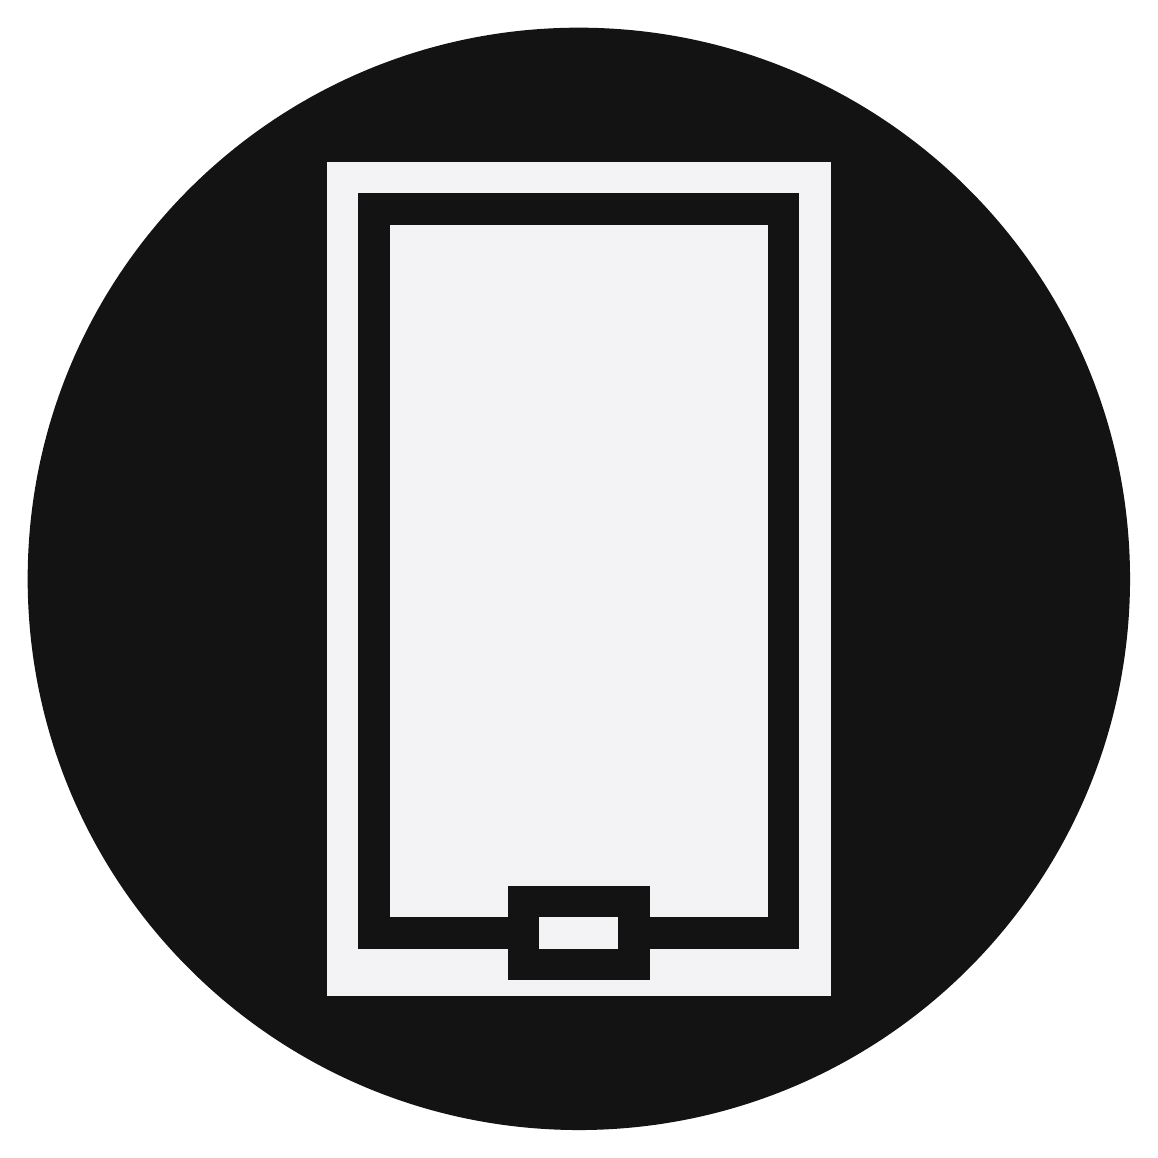
\begin{tikzpicture}
    
    % Background
    \fill[minimal-main] (0, 0) circle (7);

    % Shell
    \fill[minimal-contrast] (-3.2, -5.3) rectangle (3.2, 5.3);
    \fill[minimal-main] (-2.8, -4.7) rectangle (2.8, 4.9);
    \fill[minimal-contrast] (-2.4, -4.3) rectangle (2.4, 4.5);

    % Button
    \fill[minimal-main] (-0.9, -5.1) rectangle (0.9, -3.9);
    \fill[minimal-contrast] (-0.5, -4.7) rectangle (0.5, -4.3);

\end{tikzpicture}}}
            & \textbf{Phone} \\
                & \href{tel:+###########}{###########} \\
                & \smallspace

        \multirow{2}{*}{\scalebox{0.075}{
\begin{tikzpicture}

    % Background
    \fill[minimal-main] (0, 0) circle (7);
  
    % Foundation
    \fill[minimal-contrast] (-3.2, -5.3) rectangle (3.2, -4.7);

    % Letter
    \fill[minimal-contrast] (-2.8, -4.3) -- (2.8, -4.3) -- (2.8, -0.8) -- (0.0, -3.6) -- (-2.8, -0.8) -- cycle;
    \fill[minimal-contrast] (-2.8, -0.4) -- (0.0, -3.2) -- (2.8, -0.4) -- cycle;

    % Arrow
    \fill[minimal-contrast] (-0.8, 5.3) -- (-0.8, 2.4) -- (-1.8, 2.4) -- (0.0, 0.6) -- (1.8, 2.4) -- (0.8, 2.4) -- (0.8, 5.3) -- cycle;

\end{tikzpicture}}}
            & \textbf{E-Mail} \\
                & \href{mailto:###########}{###########} \\
                & \largespace

        & \titlefont{Personal} \\
        \hline \mediumspace

        \multirow{2}{*}{\scalebox{0.075}{
\begin{tikzpicture}
    
    % Background
    \fill[minimal-main] (0, 0) circle (7);
  
    % Foundation
    \fill[minimal-contrast] (-3.2, -5.3) rectangle (3.2, -4.7);

    % Base
    \fill[minimal-contrast] (-2.8, -4.3) -- (-2.8, -1.4) -- (0.4, -1.4) -- (0.4, -3.6) -- (1.6, -3.6) -- (1.6, -2.6) -- (2.4, -2.6) -- (2.4, -1.4) -- (2.8, -1.4) -- (2.8, -4.3) -- cycle;
    
    % Cream
    \fill[minimal-contrast] (-3.2, -1.0) -- (-3.2, 0.0) -- (3.2, 0.0) -- (3.2, -1.0) -- (2.0, -1.0) -- (2.0, -2.2) -- (1.2, -2.2) -- (1.2, -3.2) -- (0.8, -3.2) -- (0.8, -1.0) -- cycle;
      
    % Candles
    \fill[minimal-contrast] (-2.6, 0.4) rectangle (-2.0, 3.4);
    \fill[minimal-contrast] (-2.5, 3.8) rectangle (-2.1, 4.6);

    \fill[minimal-contrast] (-0.6, 0.4) rectangle (0.0, 2.2);
    \fill[minimal-contrast] (-0.5, 2.6) rectangle (-0.1, 3.4);

    \fill[minimal-contrast] (-1.4, 0.4) --  (-1.0, 0.4) -- (-1.0, 2.6) --  (-0.8, 2.6) --  (-0.8, 4.0) -- (-1.4, 4.0) -- cycle;
    \fill[minimal-contrast] (-1.3, 4.4) rectangle (-0.9, 5.2);
    
    \fill[minimal-contrast] (0.8, 0.4) rectangle (1.4, 3.6);
    \fill[minimal-contrast] (0.9, 4.0) rectangle (1.3, 4.8);
    
    \fill[minimal-contrast] (2.0, 0.4) rectangle (2.6, 2.8);
    \fill[minimal-contrast] (2.1, 3.2) rectangle (2.5, 4.0);

\end{tikzpicture}}}
            & \textbf{Date of Birth} \\
                & ########### \\
                & \smallspace

        \multirow{2}{*}{\scalebox{0.075}{
\begin{tikzpicture}

    % Background
    \fill[minimal-main] (0, 0) circle (7);

    % Foundation
    \fill[minimal-contrast] (-3.2, -5.3) rectangle (3.2, -4.7);

    % Pole
    \fill[minimal-contrast] (-2.4, -4.3) rectangle (-2.0, 4.5);
    \fill[minimal-contrast] (-2.6, 4.9) rectangle (-1.8, 5.3);
    
    % Fabric
    \fill[minimal-contrast] (-0.2, 0.8) -- (3.0, 0.8) -- (3.0, 3.9) -- (1.4, 3.9) -- (1.4, 1.2) -- (-0.2, 1.2) -- cycle; 
    \fill[minimal-contrast] (-1.6, 1.6) rectangle (1.0, 4.5);
    
\end{tikzpicture}}}
            & \textbf{Nationality} \\
                & ########### \\
                & \largespace

        & \titlefont{Platforms} \\
        \hline \mediumspace

        \multirow{2}{*}{\scalebox{0.075}{
\begin{tikzpicture}

    % Background
    \fill[minimal-main] (0, 0) circle (7);

    % Foundation
    \fill[minimal-contrast] (-3.2, -5.3) rectangle (3.2, -4.7);

    % Logo
    \fill[minimal-contrast] (1.7, -4.3) -- (-1.7, -4.3) to[out=90, in=270] (-1.675, -4.05)
                                             to[out=190, in=330] (-3.6, -3.8)
                                             to[out=150, in=330] (-4.6, -2.35) % Tail
                                             to[out=150, in=280] (-5.0, -1.9) % Tail
                                             to[out=20, in=140] (-4.0, -2.1) % Tail
                                             to[out=320, in=160] (-3.0, -3.2) % Tail
                                             to[out=340, in=210] (-1.7, -3.1) % Tail
                                             to[out=80, in=230] (-1.25, -2.2) % Shoulder (left)
                                             to[out=180, in=230, looseness=1.15] (-3.6, 3.1) % Cheek (left)
                                             to[out=110, in=250] (-3.5, 4.9) % Ear (left)
                                             to[out=340, in=130] (-1.8, 4.1) % Ear (left)
                                             to[out=15, in=165] (1.8, 4.1) % Top
                                             to[out=50, in=200] (3.5, 4.9) % Ear (right)
                                             to[out=290, in=70] (3.6, 3.1) % Ear (right)
                                             to[out=310, in=0, looseness=1.15] (1.25, -2.2) % Cheek (right)
                                             to[out=310, in=100] (1.7, -3.1) % Shoulder (right)
                                             -- cycle;

\end{tikzpicture}}}
            & \textbf{GitHub} \\
                & \href{https://github.com/gonlezmario}{gonlezmario} \\
                & \smallspace

        \multirow{2}{*}{\scalebox{0.075}{
\begin{tikzpicture}
    
    % Background
    \fill[minimal-main] (0, 0) circle (7);

    % i-base
    \fill[minimal-contrast] (-4.0, -4.0) rectangle (-2.3, 1.2);

    % i-dot
    \fill[minimal-contrast] (-3.15, 3.2) circle (1.0);

    % n
    \fill[minimal-contrast] (-1.2, -4.0) -- (-1.2, 1.2) -- (0.5, 1.2) -- (0.5, 0.5)
                 to[out=50, in=100, looseness=1.3] (4.0, -0.5)
                 -- (4.0, -4.0) -- (2.3, -4.0) -- (2.3, -0.7) 
                 to[out=100, in=80, looseness=1.1] (0.5, -0.8) -- (0.5, -4.0) -- cycle;

\end{tikzpicture}}}
            & \textbf{LinkedIn} \\
                & \href{https://www.linkedin.com/in/gonlezmario/}{gonlezmario} \\
                & \largespace

        & \titlefont{Languages} \\
        \hline \mediumspace

        \multirow{2}{*}{\scalebox{0.075}{
\begin{tikzpicture}

    % Clip mask
    \clip (0, 0) circle (7);
    
    % Red
    \fill[minimal-red] (-7, 2.4) rectangle (7, 7);

    % Yellow
    \fill[minimal-yellow] (-7, -2.4) rectangle (7, 2.4);
    
    % Red
    \fill[minimal-red] (-7, -7) rectangle (7, -2.4);
    
\end{tikzpicture}}}
            & \textbf{Spanish} \\
                & Native \\
                & \smallspace

        \multirow{2}{*}{\scalebox{0.075}{
\begin{tikzpicture}

    % Clip mask
    \clip (0, 0) circle (7);

    % Background
    \fill[minimal-blue] (0, 0) circle (7);

    % Diagonal
    \fill[minimal-white, rotate around={38.5:(0, 0)}] (-7.5, -1.1) rectangle (7.5, 1.1);
    \fill[minimal-red, rotate around={38.5:(0, 0)}] (0.0, 0.2) rectangle (7.5, 0.9);
    \fill[minimal-red, rotate around={38.5:(0, 0)}] (-7.5, -0.9) rectangle (0.0, -0.2);
    
    \fill[minimal-white, rotate around={-38.5:(0, 0)}] (-7.5, -1.1) rectangle (7.5, 1.1);
    \fill[minimal-red, rotate around={-38.5:(0, 0)}] (0.0, 0.2) rectangle (7.5, 0.9);
    \fill[minimal-red, rotate around={-38.5:(0, 0)}] (-7.5, -0.9) rectangle (0.0, -0.2);
    
    % Cross
    \fill[minimal-white] (-7.5, -1.8) rectangle (7.5, 1.8);
    \fill[minimal-white] (-1.8, -7.5) rectangle (1.8, 7.5);

    \fill[minimal-red] (-7.5, -1.25) rectangle (7.5, 1.25);
    \fill[minimal-red] (-1.25, -7.5) rectangle (1.25, 7.5);

\end{tikzpicture}
}}
            & \textbf{English} \\
                & Proficient \\
                & \smallspace

        \multirow{2}{*}{\scalebox{0.075}{
\begin{tikzpicture}

    % Clip mask
    \clip (0, 0) circle (7);

    % Red
    \fill[minimal-red] (-7, -2.4) rectangle (7, 2.4);
    
    % Black
    \fill[minimal-black] (-7, 2.4) rectangle (7, 7);
    
    % Yellow
    \fill[minimal-yellow] (-7, -7) rectangle (7, -2.4);
    
\end{tikzpicture}
}}
            & \textbf{German} \\
                & Fluent \\
                & \smallspace

        \multirow{2}{*}{\scalebox{0.075}{
\begin{tikzpicture}

    % Clip mask
    \clip (0, 0) circle (7);

    % White
    \fill[minimal-white] (-2.4, -7) rectangle (2.4, 7);
    
    % Red
    \fill[minimal-red] (2.4, -7) rectangle (7, 7);
    
    % Blue
    \fill[minimal-blue] (-7, -7) rectangle (-2.4, 7);
    
\end{tikzpicture}}}
            & \textbf{French} \\
                & Beginner

    \end{tabular}}

% -- Aboutbox
\posterbox[
    colback=white,
    valign=center,
    top=\inboxspacing,
    halign=left,
    right=\inboxspacing]
    {name=aboutbox,
    below=headbox,
    column*=1,
    span=\mainboxwidth,
    rowspan=\aboutboxheight}
{
    \textbf{Passionate electronics engineer with a keen interest in embedded systems, clean code practices, hardware design, and control engineering.}
}

% -- Mainbox
\posterbox[
    colback=white,
    valign=top,
    top=\inboxspacing,
    halign=left,
    left=\inboxspacing]
    {name=mainbox,
    column*=1,
    span=\mainboxwidth,
    below=aboutbox,
    rowspan=\mainboxheight}
{
    \begin{tabular}{>{\footnotesize}rl}
        & \titlefont{Work Expericence} \\
        \hline \mediumspace

        11/2022 - Currently
            & \textbf{Solexperts AG} \\
            & \textbf{Software Developer} \\
            & IoT platform development and maintenance \\
            & Data acquisition software development \\
            & Software migration and update \\
            & \smallspace

        04/1818 - 08/1826
            & \textbf{Nippon Gases} \\
            & \textbf{Engineering Intern} \\
            & Write and translate technical internal documentation\\
            & Requirements-Engineering \\
            & \largespace

        04/1818 - 08/1826
            & \textbf{CID Kids} \\
            & \textbf{It Teacher} \\
            & Introduced coding and electronics to children\\
            & and teenagers during a summer tech camp \\
            & Prepared lectures and electronic circuits \\
            & \largespace

        & \titlefont{Education} \\
        \hline \mediumspace

        2017 - 2022
            & \textbf{University of Oviedo} \\
            & \textbf{Industrial Electronic and Automatic Engineering} \\
            & Bilingual Itinerary (240 ECTS)\\
            & Energy Efficient Electronics Especialization\\
            & \smallspace

        2019 - 2020
            & \textbf{Liverpool John Moores University} \\
            & \textbf{Electrical and Electronic Engineering} \\
            & Erasmus+ Scholarship \\
            & First Honours \\
            & \largespace
    \end{tabular}
    
    \begin{tabularx}{\textwidth}{Xl}
    \titlefont{Soft Skills} & \titlefont{Hard Skills} \\
    \hline \mediumspace
    Communication & Python \\
    Problem-Solving & C/C++ \\
    Flexibility & IoT \\
    Attention to Detail & PCB Design \\
    Continuous Learning & Linux \\
    \smallspace
\end{tabularx}
}

% -- Footbox
\posterbox[colback=minimal-main]
           {name=footbox,
           below=sidebox,
           span=1,
           rowspan=\footboxheight}{}

\end{tcbposter}
\end{document}
